\chapter{Compliance jako klíčový parametr pandemie}
\label{Compliance}

\textit{Jan Kulhánek, Lucie Michálková, Josefína Weinerová}
\vspace{15mm}

\section*{Úvod} 

Od začátku pandemie onemocnění covid-19 se naše země potýká při snaze situaci zvládnout s~organizačními a komunikačními problémy \cite{CeskaTiskovaKancelar2020,Vlckova2020}. Jedním ze stěžejních faktorů efektivního boje s~pandemií je compliance -- dodržování protiepidemických opatření širokou veřejností \cite{VanRooij2020}. Náš článek nabízí rozbor psychologických faktorů, které mohou míru compliance ovlivnit. Opíráme se při tom o~teorie z~kognitivní psychologie, sociální psychologie, vlastní šetření a veřejně dostupná data. 

Účinnost preventivních opatření, jako je mytí rukou, nošení roušek, sociální distancování apod. záleží na míře jejich dodržování, tzv. compliance. Zvláště ve druhé a třetí vlně pandemie se u~nás objevilo přibývající množství zpráv o~jejich nedodržování. Například data z~ČR z~podzimu 2020 ukazují, že zatímco lidé při trasování oficiálně hlásí hygieně jeden rizikový kontakt týdně (viz kapitolu \ref{Trasovani}), anonymně přiznávají 4--7 kontaktů \cite{tr_PAQ01}. Navíc podle sociologického šetření Život během pandemie z~listopadu 2020 bylo mezi dospělými respondenty až 12 \% tzv. rizikových netestovaných, tedy lidí, kteří měli v~posledním měsíci buď kontakt s~nakaženým, nebo příznaky covid-19 a zároveň v~té době nebyli testováni \cite{Prokop2020a}. Malá míra otestovanosti může indikovat i to, že tito lidé (a jejich kontakty) nejsou hygieně známi. Nedodržování opatření není zdaleka jen problém České republiky, podle reportů z~Harris County v~USA ze srpna 2020 odmítlo 25 \% z~nakažených lidí kontaktovaných během trasování nahlásit jakékoli rizikové kontakty \cite{Shapiro2020}. A~třeba dotazníková studie ve Velké Británii odhalila, že jen 20 \% lidí dotázaných mezi dubnem 2020 a lednem 2021 během nařízené izolace skutečně neopustilo místo bydliště \cite{Smith2021}.

Jedním z~preventivních chování, které může výrazně ovlivnit další průběh pandemie, je také ochota nechat se očkovat. Data sesbíraná na reprezentativním vzorku respondentů z~Velké Británie a Irska na jaře 2020 ukazují, že 31 \% (Velká Británie) a 35 \% (Irsko) respondentů se buď nehodlalo nechat naočkovat, nebo se spíše přikláněli k~tomu, že se očkovat nenechají \cite{Murphy2021}. Podle sociologického výzkumu Život během pandemie provedeného na českém vzorku by se ke 4. květnu 2021 rozhodně nebo spíše nenechalo očkovat 24 \% respondentů \cite{Prokop2021}.

Subjektivní postoje jednotlivců vůči individuálním preventivním opatřením nevyhnutelně ovlivní, zda budou jedinci opatření dodržovat či nikoli. Proto je při řešení problematiky compliance důležité také přihlédnout k~faktorům, které mohou tyto subjektivní postoje ovlivňovat. V~rámci tohoto článku prezentujeme výsledky tří šetření mapujících spolupráci během trasování a preference seniorů týkající se místa očkování. V~Diskusi pak popisujeme, jak lze získané výsledky rozebrat v~kontextu uznávaných teorií ze sociální a kognitivní psychologie včetně teorie plánovaného chování.

\section*{Metody} 

Pro zkoumání compliance v~českém prostředí jsme zvolili konkrétní témata, která podle nás dobře ukazují příležitosti pro zvyšování compliance: 

\begin{enumerate}
\item Prvním tématem bylo vnímání spolupráce s~hygienickými stanicemi, kde jsme zkoumali rozměr osobního postoje ke spolupráci a důvody nehlášení rizikových kontaktů. 
\item Druhé téma se zaměřuje na aspekty omezeného využívání eRoušky.
\item Třetím tématem bylo zkoumání nízké motivace seniorů nechat se očkovat v~očkovacích centrech. Během jara 2021 jsme opakovaně pozorovali zájem lidí o~očkování u~praktických lékařů, kterého nebylo plně využito. Aspektem zkoumání byla specifika subjektivní kontroly cílové skupiny a především limity, kvůli kterým tato skupina preferuje očkování u~praktického lékaře před jinými očkovacími místy.
\end{enumerate}

Prvnímu a druhému výzkumu dominoval přístup kvantitativní - data byla sbírána nejdříve v~rámci pilotního online šetření a následně v~rámci projektu Život během pandemie na reprezentativním vzorku. Třetí šetření bylo uchopeno kvalitativně.

\section*{Téma 1 a 2 – Kvantitativní šetření hlášení rizikových kontaktů a využívání eRoušky}
\paragraph*{Metody.}
Laboratoř veřejných politik BISOP se pravidelně věnovala rychlosti trasování dostupné z~dat Ministerstva zdravotnictví ČR, které bylo předmětem pravidelných monitoringů \cite{Blechova,Blechova2020}. Data jsme chtěli doplnit o~kvalitativnější část, a proto jsme nejdříve skrze sociální média rozšířili anonymní dotazník zaměřený na zkušenosti s~hygienickými stanicemi, především na postoje k~nástrojům testování a trasování. Jednalo se o~explorativní šetření, které mělo podpořit další zkoumání compliance. Set byl tvořen devíti otázkami zaměřenými na kontakt s~hygienickou stanicí, na využívání trasování, sebereportování i pomocných nástrojů typu eRouška \cite{Erouska.cz2020}. Vzorek respondentů nebyl reprezentativní (dotazník byl šířen přes facebookový účet BISOP a naše osobní profily). Šlo především o~respondenty, které se nám podařilo oslovit v~rámci našich kontaktů na sociálních sítích. 
Díky tomuto pilotnímu šetření jsme formulovali set otázek, který byl zařazen ve sběru dat „Život během pandemie“ v~květnu 2021, kdy společnost PAQ \cite{Prokop2021a} naše dílčí otázky k~trasování zakomponovala do svého pravidelného telefonického sociologického výzkumu a díky tomu se naše otázky dostaly k~reprezentativnímu vzorku 1975 respondentů. 
Z~nich mělo s~trasováním zkušenost 274 lidí. Těmto respondentům byly položeny stejné otázky, které jsme pokládali již v~rámci prvního šetření o~trasování. Respondenti pak měli vybrat vždy jednu z~nabízených možností (na vybranou měli volit z~2--5 odpovědí). 

%\subsection*{Výsledky}
\paragraph*{Výsledky pilotního šetření k~tématu trasování.}
Z~našeho šetření na sociálních sítích vyplývá, že rozhovor s~hygienou je vnímán jako bezproblémový naprostou většinou respondentů, kteří dotazník vyplnili. Dále hodnotili rozhovor jako profesionálně vedený. Pracovníci a pracovnice hygienických linek za uplynulé měsíce odvádějí dobrou práci. Tři ze čtyř dotazovaných uvádějí, že telefonát šel hladce, svižně. Hygiena se téměř polovině nakažených ozve už během prvních 24 hodin po testu, případně po nahlášení rizikového kontaktu a celkově lze s~jistotou vyvrátit obavy, že se lidé telefonátu od hygieny nedočkají.

Možnost sebereportování prozatím užívá jen velmi omezené množství lidí – v~na\-šem drobném šetření na sociálních sítí ho využila jen jedna třetina respondentů. Polovina respondentů o~této možnosti dokonce ani nevěděla. 

Ještě méně lidí v~našem šetření pak aktivně využívá aplikaci eRouška, zhruba každý čtvrtý. Třetina dotazovaných dokonce uvedla, že používali eRoušku dříve, ale aplikaci si odinstalovali.

\pagebreak
\begin{figure}[h!]
\begin{center}
    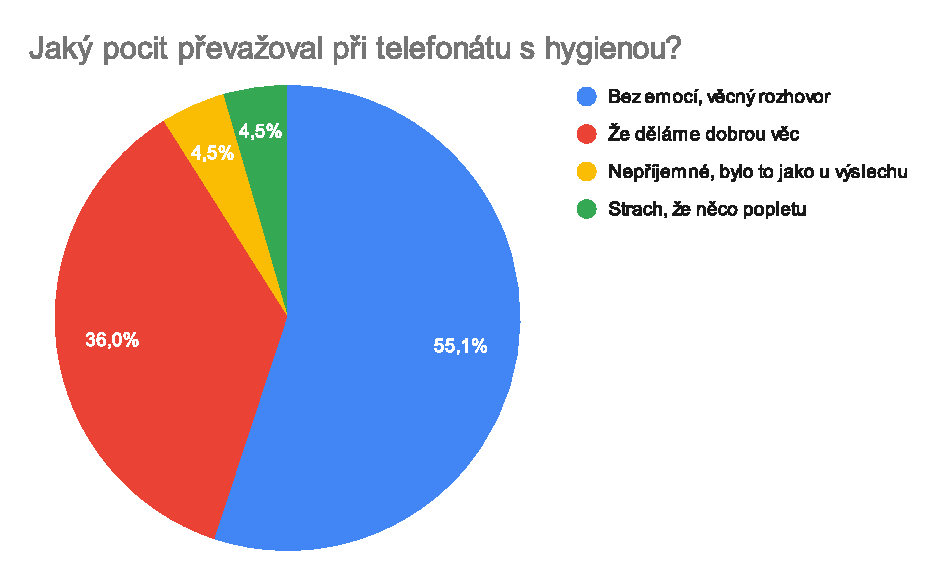
\includegraphics[width=250pt]{./pic/graf1.eps}
\end{center}    
% \textit{Graf 1 ukazuje procentuální podíl odpovědí na otázku o převládajících pocitech z telefonátu  hygienou. Většina respondentů měla z telefonátu buď pozitivní pocity, nebo ho zhodnotila jako věcný.}
\caption{Procentuální podíl odpovědí na otázku o~převládajících pocitech z~telefonátu  hygienou. Většina respondentů měla z~telefonátu buď pozitivní pocity, nebo ho zhodnotila jako věcný (data z pilotního šetření).}
 \end{figure}
\begin{figure}[h!]
\begin{center}
    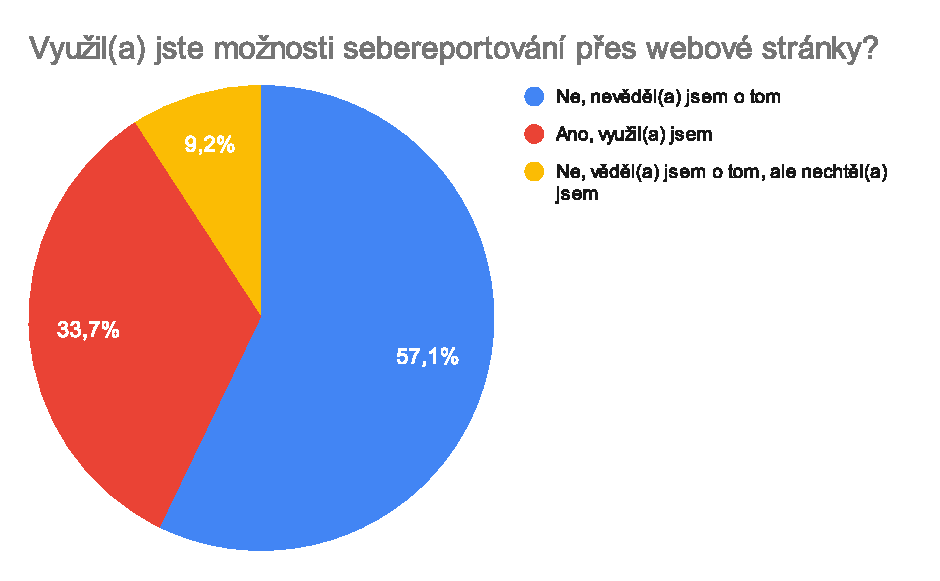
\includegraphics[width=250pt]{./pic/graf2.eps}
 \end{center}    
    \caption{Procentuální podíl odpovědí na otázku o~využívání nástroje pro sebereportování. Většina respondentů o~této on-line aplikaci nevěděla (data z pilotního šetření).}
\end{figure}
\begin{figure}[h!]
\begin{center}
    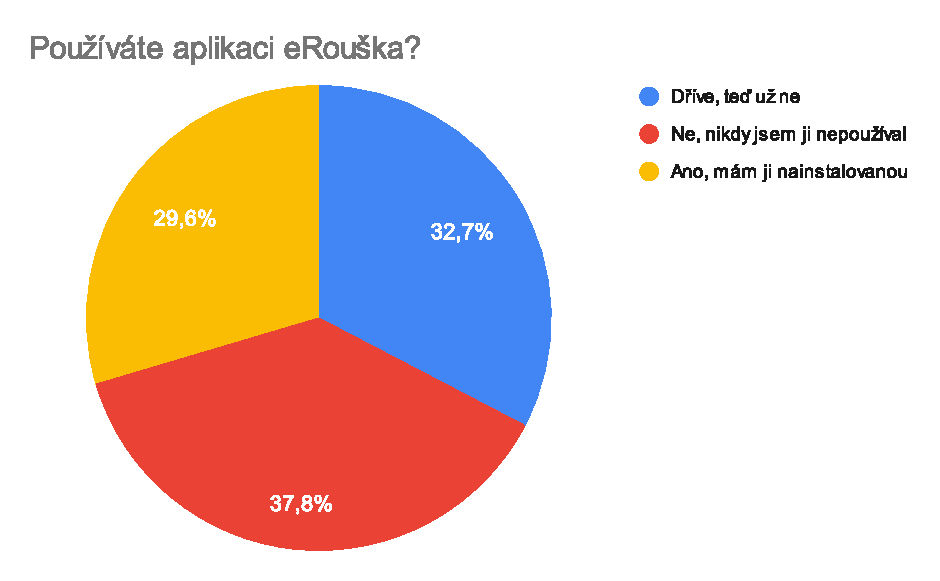
\includegraphics[width=250pt]{./pic/graf3.eps}
 \end{center}    
%    \textit{Graf 3 ukazuje procentuální podíl odpovědí na otázku o používání aplikace eRouška. Většina respondentů aplikaci nepoužívá, třetina dotázaných používala dříve.}
\caption{Procentuální podíl odpovědí na otázku o~používání aplikace eRouška. Většina respondentů aplikaci nepoužívá, třetina dotázaných používala dříve  (data z pilotního šetření).}
 \end{figure}
 
\pagebreak
\paragraph* {Výsledky odpovědí v~rámci výzkumu Život během pandemie.}
Ze vzorku 1975 respondentů pro sociologický výzkum „Život během pandemie“ mělo s~komunikací s~krajskou hygienickou stanicí (dále KHS) zkušenost 14 \% osob. 57 \% z~nich se KHS ozvala do 24 hodin, 76 \% do 48 hodin. Starším lidem se KHS ozvala v~68 \% do 24 hodin, naopak lidem do 34 let jen ve 32 \% případů. 

Telefonát nebyl stresující pro naprostou většinu respondentů -- 76 \% respondentů uvádí, že byli zcela bez nervozity, dalších 18 \% popisuje nervozitu jen ze začátku telefonátu. 58 \% dotazovaných se zdál rozhovor věcný, bez emocí, pro dalších 26 \% byl telefonát doprovázen pocitem, že dělají dobrou věc. Častěji zažívají u~trasování pocit, že dělají dobrou věc, ti lidé, kteří znají někoho, kdo na covid-19 zemřel, a starší lidé.

Dalším okruhem výzkumu bylo nevyužívání hlášení kontaktů a jeho důvody. 72 \% respondentů odpovědělo, že při telefonátu uvedlo všechny osoby, se kterými byli v~kontaktu, 14 \% odpovědělo, že neví. 

U~14 \% dotazovaných, tedy 31 lidí, kteří odpověděli, že při telefonátu s~KHS neuvedli všechny osoby, se výzkum dále ptal na jejich důvody, proč kontakty neuvedli (možno bylo uvést více možností). Nejpočetnější -- 28 \% uvedlo, že si v~té chvíli na všechny své kontakty nevzpomněli, neboť bylo málo času. Ostatní důvody jsou shrnuty v~Tabulce 1.

\begin{table}
\begin{center}
\begin{tabular}{|l|r|}
\hline
\emph{Důvody pro neuvedení všech kontaktů při trasování (N=31)} &  \% \\
\hline \hline
Na všechny kontakty si v~té chvíli nevzpomněli & 28\% \\
Nevěděli jméno či kontaktní údaje kontaktu & 24\% \\
Nechtěli, aby dotyčný šel do karantény a přišel o~příjem z~práce & 21\% \\
Domluvili se s~dotyčným kontaktem, že se nahlásí sám & 20\% \\
Nevěděli, zda by s~tím dotyčný souhlasil & 17\% \\
Zaměstnavatel si nepřál, aby hlásili lidi z~pracoviště & 12\% \\
Cítili tlak ze strany hygieny, aby neuváděli příliš mnoho kontaktů & 10\% \\
Dotyčný kontakt již měl covid nebo je naočkovaný & 9\% \\
Nevěří trasování a hygieně & 6\% \\
Jiné důvody & 10\% \\
\hline
\end{tabular}
\end{center}
%\textit {Tabulka 1 shrnuje důvody respondentů (N=31) pro neuvedení všech kontaktů během trasování. Respondenti mohli zvolit než jednu možnost.}
\caption{Důvody respondentů (N=31) pro neuvedení všech kontaktů během trasování. Respondenti mohli zvolit více než jednu možnost.}
\end{table}

\paragraph*{Využívání e-nástrojů sebetrasování a eRoušky.}
O~využívání nástroje sebereportování před samotným telefonickým rozhovorem stále neví 49 \% respondentů. Pouze 23 \% respondentů možnosti sebereportování využilo. Z~těch, kteří možnost sebereportování využili, se 71 \% přiklání k~tomu, že to při telefonickému rozhovoru pomohlo -- rozhovor byl díky tomu svižnější nebo lidé informace jen rychle zopakovali. Znalost sebereportování je velmi závislá na věku -- nad 55 let věku ji 70 \% lidí nezná. 

Poslední otázka kopírující náš předchozí výzkum se týkala využívání aplikace eRouška -- jen 15 \% z~celkových 1975 respondentů uvedlo, že má nainstalovanou aplikaci eRouška. Shodně 15 \% uvedlo, že tuto aplikaci měli nainstalovanou dříve, nyní ne. 70 \% respondentů ji nepoužilo nikdy. Lidé do 34 let si eRoušku často smazali z~mobilu. 

\section*{Diskuse}
\paragraph*{Psychologické hypotézy o~nižší compliance při trasování.}
Spokojenost účast\-ní\-ků s~průběhem a kvalitou trasování je v~kontrastu s~tím, že lidé při trasování hlásí výrazně méně kontaktů, než by indikovala data ze sociologických průzkumů \cite{Prokop2020a}. V~této sekci představujeme možné psychologické přístupy, skrze něž se dá na výše uvedená data a problematiku compliance nahlížet.  

Jedna ze styčných psychologických teorií popisujících faktory ovlivňující chování je Teorie plánovaného chování \cite{Ajzen1985}. Tato teorie byla v~minulosti úspěšně otestována a aplikována na řadu preventivních chování, jako jsou zdravé dietní návyky \cite{Hackman2014}, mytí rukou \cite{Hackman2014} nebo řízení pod vlivem alkoholu \cite{Moan2011}. V~souvislosti s~výzkumem compliance během pandemie covid-19 byla korelace faktorů postulovaných Teorií plánovaného chování nalezena například se sociálním distancováním u~hongkongských \cite{Yu2021} a bangladéšských respondentů \cite{Das2021}. 

Tato teorie rozlišuje mezi intencí k~tomu, provést nějaké chování (například hlášení kontaktů při trasování) a chováním samotným. Intence je dále ovlivněna osobními postoji jednotlivce ke konkrétnímu chování, jeho subjektivními spo\-le\-čen\-ský\-mi normami a pocitem kontroly nad chováním. 
Vztah mezi intencí a chováním samotným je také ovlivněn reálnou kontrolou nad chováním \cite{Ajzen1985}. Interakce mezi faktory je vizualizovaná na obrázku \ref{fig:graph}. Osobní postoje, normy a pocit kontroly postulované Teorií plánovaného chování se formují na pozadí individuálních (např. osobnostní rysy, zkušenost), společenských (např. náboženství, kultura, vý\-cho\-va) a informačních vlivů (např. zprávy v~médiích). 

\begin{figure}
\begin{center}
    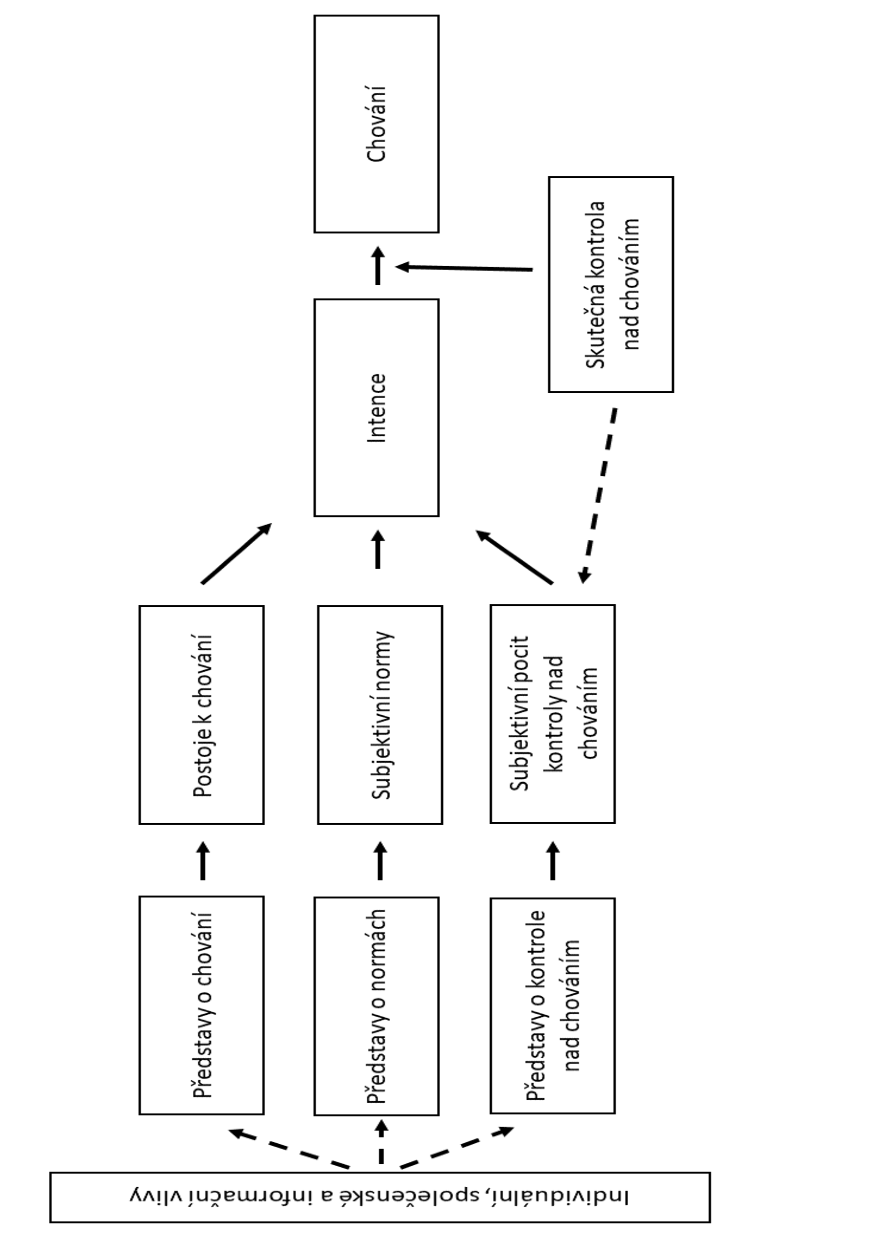
\includegraphics[angle=270,width=300pt]{./pic/Ajzen2-cs.eps}
    
    \caption{Graf ukazuje faktory ovlivňují intenci k~určitému chování podle Teorie plánovaného chování. Obrázek přeložen z~\cite{Ajzen2018}.}
    \label{fig:graph}
\end{center}
\end{figure}

Subjektivní normy jsou vytvářeny na základě informací o~tom, jak se chová většina společenské skupiny daného jedince v~interakci s~dalšími již existujícími normami \cite{Ajzen1991}. Tato představa však může být zkreslená, například kvůli relativně uzavřeným skupinám na sociálních sítích, tzv. sociálním bublinám \cite{Gonzalez-Padilla2020}. Sociální bubliny jsou propojené skupiny lidí s~podobnými názory a zájmy. To vede k~přenášení jen určitých informací. Sociální bubliny tak mohou mít negativní dopad na compliance, protože se v~nich mohou přenášet pouze informace z~určitých zdrojů, což posiluje selektivní vidění světa \cite{Gonzalez-Padilla2020,Pariser2012TheFB}. 

Jednou z~cest, jak zvýšit compliance, tedy může být navození pocitu, že většina lidí opatření dodržuje. V~kontextu trasování se může otázka na počet rizikových kontaktů dát do vztahu k~datům z~průzkumů, např.: „Data z~České republiky ukazují, že aktuální průměr je 13 kontaktů za týden. Řekl/a byste, že jste se za stejnou dobu setkal/a s~menším, nebo větším počtem lidí?“ Mimo ovlivnění subjektivní normy může tento způsob fungovat také jako forma kotvení (v~anglickém překladu anchoring), kognitivního bias, při kterém máme tendenci vztahovat (kotvit) odpovědi na určitou informaci \cite{Tversky1974}.

Také je potřeba brát v~potaz to, že jedinci si během rozhovoru s~KHS nemusí vzpomenout na všechny kontakty, na které by mohli. Zvláště když jsou při vybavování kontaktů instruováni k~použití fotek a čísel z~telefonu, který ale zároveň používají k~rozhovoru s~KHS. V~takových případech by mohlo pomoci zaslání pří\-prav\-né SMS, v~níž by byl uveden a) čas telefonátu od KHS a b) seznam informací, na které se KHS bude ptát. To by utvořilo možnost se na telefonát náležitě připravit a zároveň urychlilo celý proces.

Prostor pro šíření zastaralých informací a dezinformací bude ovlivněn také komunikační strategií ze strany autorit. Jasná komunikace aktuálního stavu pandemie a jednotlivých preventivních opatření bude tedy též hrát klíčovou roli v~míře compliance \cite{Hyland-Wood2021}. 

\paragraph*{K výsledkům trasování zjištěných díky Životu v~pandemii.}
Výsledky roz\-ší\-ře\-né\-ho výzkumu o~trasování potvrdily trendy, na které poukázalo naše prvotní šetření. Nejsilnějším výsledkem výzkumu je, že 70 \% dotazovaných nikdy nepoužívalo aplikaci eRouška. Dle Českého statistického úřadu přitom používá chytrý telefon přes 70 \% Čechů \cite{Mana2020}. Zdá se tedy, že propagace aplikace nebyla dostatečná. To ukazují i data z~Chytré karantény: v~říjnu 2020 aplikaci používal pouze jeden milion lidí (tedy cca 10 \% obyvatel ČR) \cite{Fiser2020}. Větší propagaci by si zasloužila i možnost sebereportování přes webové stránky, polovina respondentů o~ní nevěděla a jen 23 \% respondentů ji využilo. Sebereportování přitom ulehčuje proces trasování oběma stranám. 

Zvláštní pozornost si zaslouží i interpretace dat spojených s~nehlášením rizikových kontaktů KHS. Dva nejčastější důvody, proč lidé kontakty nehlásí, jsou, že si lidé nevzpomněli na všechny své kontakty, případně si nepamatovali jejich jméno či kontaktní údaje. Přitom by právě tyto těžkosti šlo překonat využitím sebereportovacího protokolu -- jedinec by byl veden k~tomu, aby vybavování pomohl na základě svého diáře, fotek z~telefonu či komunikace s~přáteli a následně se může snáz pokusit potřebné informace doplnit. Tato data potvrzují přínos sebereportování.

\subsection*{Poznámky k~nástrojům Sebereportování a eRouška.}
Přes polovinu dotazovaných o~možnosti sebereportování vůbec nevědělo. Nízké vy\-uži\-tí této možnosti hlášení rizikových kontaktů potvrzují i statistiky krajských hygienických stanic. Např. podle reportu Ministerstva zdravotnictví ČR z~26. března využilo sebetrasování 10–15 \% pozitivních \cite{MinisterstvoZdravotnictviCR2021}. Možnost sebereportování má potenciál zkrátit rozhovor s~hygienickou stanicí, tudíž šetří čas oběma stranám. Navíc funkční sebereportování podporuje důvěru ve spolupráci s~veřejnou institucí, což občanům chybí. Podle našeho názoru by si proto webová aplikace zasloužila daleko více propagace, než se jí dostává. Pro ty, kteří jsou zvyklí vyřizovat záležitosti on-line, by se mělo jednat o~primární cestu trasování. 
V~době, kdy je epidemie ještě silná, může být mnoho výhrad vůči eRoušce oprávněných, ať už jde o~možnost falešně pozitivních hlášení (eRouška ohlási i kontakt, při kterém měly obě strany respirátor) nebo to, že hlášení eRoušky negeneruje automaticky žádanku na test. Ve stavu, kdy se budou vyskytovat pouze jednotky nakažených, však něco jako eRouška může nabýt na významu. Jejích varování bude velice málo, takže lidem nebude zatěžko jít se testovat, a státu nebude zatěžko v~oněch případech testování zdarma umožnit. 
Většina občanů v~produktivním věku je zvyklá využívat v~komunikaci se státem elektronickou formu – například je u~nás přes milion zřízených datových schránek \cite{DatoveSchranky2021}. U~této skupiny se nabízí větší propagace uvedených elektronických nástrojů ke zvládání epidemie. U~dominantně starší skupiny obyvatel, kteří na elektronickou komunikaci se státem nejsou zvyklí, doporučujeme podporovat možné mezistupně v~komunikaci – pomocníka či mediátora, který starším občanům a občankám pomůže. Tuto roli mohou plnit nejen děti a vnoučata, ale i pojišťovny nebo komunitní skupiny. 

\section*{Téma 3 - Kvalitativní šetření důvodů pro demotivaci seniorů nechat se očkovat v~očkovacích centrech}

\paragraph*{Metody.}
Třetí výzkum se zaměřoval na pochopení důvodů, kvůli nimž respondenti preferují očkování u~praktického lékaře před nabízenými očkovacími místy. Pro výzkum jsme uspořádali šetření formou kvalitativních rozhovorů s~respondenty, kteří nadále čekají na možnost očkování u~praktického lékaře, ačkoli by již mohli být očkováni v~očkovacích centrech. Oslovili jsme celkem 23 respondentů, z~toho 15 seniorů a 8 rodinných příslušníků. Výběr respondentů probíhal na sociálních sítích. V~semistrukturovaných rozhovorech jsme zkoumali důvody, proč se respondenti ještě neregistrovali k~očkování v~rezervačním systému. Zajímalo nás, co je ve vztahu k~očkování v~očkovacích centrech demotivuje i jaké jsou jejich motivace k~očkování u~praktického lékaře. Vzhledem k~malému a nereprezentativnímu vzorku jde o~orientační výstup. 
 
\paragraph*{Výsledky.}
V~kvalitativním šetření týkajícím se motivace k~očkování jsme se v~rozhovorech zaměřili na důvod preference seniorů očkovat se u~praktických lékařů. Odpovědi vykazovaly značnou míru konzistence a lze z~nich vysledovat několik jasných postojů a obav.
V~odpovědích respondentů se opakovala větší obeznámenost praktického lékaře s~osobní i rodinnou anamnézou jedince. „Obvodní lékař zná dobře náš zdravotní stav, důvěřujeme mu ohledně případných komplikací po očkování, o~kterých se všude píše…“ Praktický lékař je seznámen se stavem jedince a konečnou odpovědnost za správné vyplnění formuláře a vyloučení kontraindikací před očko\-vá\-ním nenese jen očkovaný. 
Dalším odrazujícím faktorem je pro řadu lidí neznámé prostředí a organizační nároky spojené s~cestou na očkovací místo. „Svého doktora mám v~docházkové vzdálenosti, nemusím zbytečně cestovat MHD nebo obtěžovat své děti, aby mě dovezly.“ Při rozhodování je relevantní obava z~toho, že se jedinec na rušném místě nakazí: „Raději si počkám na očkování u~svého obvodního lékaře, protože se bojím, abych se v~nemocnici sama covidem nenakazila…“
Od organizace k~očko\-vá\-ní ve velkokapacitním místě pak seniory odrazují komplikace spojené s~telefonováním. „Nepamatuji si, na co beru léky, nechci kvůli tomu volat obvoďákovi a pak to vyplňovat na papíru k~očkování.“ Telefonické konzultace s~praktikem a odpovědnost za správné vyplnění všech formulářů ve velkokapacitním centru vnímají senioři jako problém. Jako další problém uvádějí senioři shlukování velkého množství lidí, na které si za doby pandemie dále odvykli. „Z nemocnice mám obavy, určitě tam bude hodně lidí. U~svého praktika to znám.“ Často navíc osoby k~praktikovi docházejí pravidelně pro léky či na kontrolu, a očkování by se tedy spojilo s~již naplánovanou kontrolou.

\section*{Diskuse}

\paragraph*{K výsledkům kvalitativního šetření k~očkování seniorů.}
Z~výsledků našeho šetření vyplývá, že preference respondentů nechat se očkovat u~praktického lékaře byla ovlivněna především důvěrou a pocitem bezpečí. V~březnu/dubnu 2021 k~nám z~médií přicházely negativní zprávy o~možných zdravotních komplikacích spojených s~očkováním \cite{Svamberk2021,MinisterstvoZdravotnictviCR2021a}. Je samozřejmě důležité, aby byla ve\-řej\-nost informovaná, ovšem zjednodušující výstupy vytržené z~kontextu vyvolávají emoce strachu a zejména u~seniorů snižují důvěru v~bezpečí očkování jako takového. Přitom čísla mluví jasně – rizika spojená s~očkováním jsou nesrovnatelně nižší než rizika spojená s~onemocněním \cite{Statniustavprokontroluleciv2021}. 
To může ovlivnit jak osobní postoje seniorů vůči očkování, tak jejich subjektivní pocit kontroly nad tím, se k~očkování reálně dostavit. Praktický lékař pro seniora představuje větší záruku bezpečí než anonymní systém, který se potýká s~nedůvěrou a kritikou velké části společnosti. Pokud tedy praktický lékař osobně zavolá svému pacientovi, po zvážení jeho anamnézy ho pozve k~očkování a dá mu navíc brzký termín, výrazně to zvyšuje šanci na úspěšnou vakcinaci seniorů.
Respondenti uváděli také jako jeden z~faktorů strach z~jízdy v~MHD, kde se potenciálně mohou nakazit. Tento strach může ovlivnit subjektivní pocit kontroly nad schopností na očkování reálně dorazit. Intervence zaměřená na snížení tohoto rizika tedy může také zvýšit šanci na vakcinaci. Například v~Německu se rozhodli podpořit seniory tím, že jim poskytují při cestě za očkováním taxi za cenu běžné jízdenky, navíc je chrání darovaným FFP2 respirátorem \cite{Kreijger2021}.

\section*{Limitace výzkumu}

Vzhledem k~tomu, že jak pilotní šetření trasování, tak šetření k~očkování probíhala on-line a byla šířena přes sociální média, respondenti budou pravděpodobně pravidelnými uživateli sociálních sítí. To může vést k~nadhodnocení počtu lidí používajících jiné on-line metody (například sebereportování a aplikaci eRouška). 
Vzorek navíc nebyl reprezentativní vůči populaci, většina respondentů byla z~Prahy a pravděpodobně pocházejí ze sociálních bublin autorů článku.
Tyto limitace jsou nicméně do velké míry v~případě trasování překonány daty z~výzkumu PAQ \cite{Prokop2021a}.
Náš výzkum nazírá na problematiku compliance z~psychologického hlediska, tím se ovšem nesnažíme tvrdit, že neexistují i jiné, nepsychologické faktory, které mohou compliance ovlivnit (např. finanční zázemí). Tyto faktory nebyly předmětem naší studie.


\section*{Výhledy do budoucna }

Ačkoli se tento článek zabýval compliance s~konkrétními preventivními opatřeními proti covid-19, přístupy, které zde prezentujeme, se dají aplikovat i v~rámci preventivních opatření proti jiným nemocem či chováním. Proto se naše doporučení dají potenciálně využít i v~rámci jiných zdravotních krizí, ne jen té současné. Ze všeobecného hlediska je užitečné vzít v~úvahu faktory ovlivňující subjektivní normy a postoje jedinců k~danému chování a zároveň se snažit snížit strukturální a fyzické bariéry, které mohou zamezit určitému kýženému chování. 

\section*{Závěr}

Naše psychologicky zaměřené zkoumání compliance v~průběhu pandemie covid-19 vneslo do popředí nevyužité příležitosti při trasování i očkování. Nevyužitou pří\-le\-ži\-tos\-tí při trasování zůstávají digitální nástroje trasování -- především sebereportování skrze webovou stránku a využívání e-Roušky pro rychlejší trasování. V~podpoře očkování se jako málo využívaní zprostředkovatelé v~rámci zdravotního systému jeví praktičtí lékaři, u~kterých deklarovala zájem se očkovat část dosud neočkovaných jedinců. Na základě výzkumu můžeme konstatovat, že hygienické stanice jsou vnímány věcně, profesionálně a telefonáty za účelem trasování nejsou pro respondenty stresující. 

\section*{Poděkování}

Za spolupráci s~PAQ velmi děkujeme. Díky tomu se naše otázky dostaly k~reprezentativnímu vzorku téměř 2000 respondentů a respondentek. Výsledky pak mohly lépe vystihnout zkušenosti a pocity obyvatel České republiky.